\newcommand{\RV}{Random Variable } 
\newcommand{\rv}{random variable } 
\chapter{Discrete \RV}

\section{Basic Concepts}
Given an experiment and a set of possible outcomes (sample space), a \rv associates a particular number with each outcome. Thus, \textbf{ a \RV is just a function from outcomes to $\Re$}. The associated numerical value is simply called as the value of the \rv.

\begin{figure}[h]
   \center
   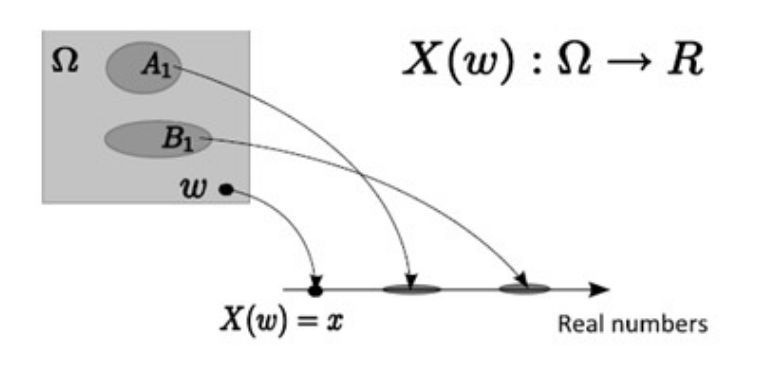
\includegraphics[width=.6\textwidth]{images/P_random_variable.jpg}
   \captionsetup{width=0.7\textwidth}
   \caption{Visualization of a \RV as a mapping from outcomes to a numerical value}
\end{figure}

\begin{definition}
    A \rv is a real-valued function of the outcome of the experiment.
\end{definition}

\subsection{Main concepts related to \rv}
Starting with a probabilistic model of an experiment:
\begin{itemize}
    \item A function of a \rv defines another random variable.
    \item A \rv can be associated with certain \textit{averages} of interest: mean and variance.
    \item A \rv can be conditioned on an event or another random variable.
    \item Notion of independence of a \rv with another \rv or an event.
\end{itemize}

\begin{definition}
    A \rv is called \textbf{discrete} if the set of values that it takes is finite or countably infinite.
\end{definition}

\subsection{Concepts related to Discrete \RV}
Starting with a probabilistic model of an experiment:
\begin{itemize}
    \item A discrete \rv has an associated probability mass function (PMF) which gives the probability of each numerical value that the \rv can take.
    \item A function of a discrete \rv defines another discrete \rv whose PMF can be obtained from the PMF of the original random variable.
\end{itemize}

This chapter will only exercise notation of the concepts that we've already studied previously (conditioning, independence, etc.) and the only new concept will be the mean and the variances.

\section {Probability Mass Function}
A PMF for a \rv $X$, is denoted by $p_X(x)$ is the probability of the event $\{X=x\}$, consisting of all outcomes that give rise to a value of $X$ equal to $x$:
\[p_X(x)=P(\{X=x\})\]

We'll avoid writing braces for brevity and use upper case characters for \RV and lower case characters for the values that the \rv can take.

We have $\sum_x p_X(x)=1$, where $x$ ranges for all values of the \rv $X$. Similarly for any set $S$ of possible values of $X$ 
\[P(X \in S) = \sum_{x\in S} p_X(x)\].

\subsection{Calculation of PMF of a \RV $X$}
For each possible values $x$ of $X$
\begin{enumerate}
    \item Collect all possible outcomes that give rise to event $\{X=x\}$
    \item Add their probabilities to obtain $p_X(x)$
\end{enumerate}

\section{Functions of a \RV}
If $Y=g(X)$ is a function of a rv $X$, then $Y$ is also a \rv since it provides a numerical value for each possible outcome. If $X$ is a discrete \rv then $Y$ is also a discrete \rv and its PMF can be calculated using PMF of $X$. 

In particular, to obtain $p_Y(y)$ for any $y$, we add the probabilities of all values $x$ such that $g(x)=y$
\[p_Y(y)=\sum_{x|g(x)=y}p_X(x)\]

\section{Expectation, Mean, Variance}
\subsection{Expectation}
\begin{definition}
    The expected value (also called as mean or expectation) of a \rv X with PMF $p_X(x)$ is 
    \[ \boxed{\E[X] = \sum_x x \, p_X(x)}\]
\end{definition}

Expectation can be thought of as a weighted average of all possible values of a \rv $X$. Analogously expected value corresponds to the \textit{centre of gravity} of the PMF.

\subsection{Variance, Moments and the Expected Value Rule}
We define the $n^{th}$ moment as $\E[X^n]$, the expected value of the \rv $X^n$. The first moment is just the mean.

Another interesting quantity is variance which is denoted by var($X$) and is defined as the expected value of $(X-\E[X])^2$, i.e.,
\[\text{var}(X) = \E[(X-\E[X])^2]\]
The variance is the measure of dispersion of $X$ around its mean. Another measure is standard deviation which is defined as the square root of the variance and is denoted by 
\[\sigma_X = \sqrt{\text{var}(X)}\]

\subsubsection{Expected Value Rule for Function of \RV}
Let $X$ be a \rv and let $g(X)$ be a function of $X$. Then the expected value of the \rv $g(X)$ is
\[\E[g(X)] = \sum_x g(x) p_X(x)\]

This allows us to avoid calculating the PMF of $g(X)$ and use the PMF of the original \rv

Using the above rule var($X$) is

\[\text{var}(X) = \sum_x (x-\E[X])^2 p_X(x)\]
Similarly, the $n^{th}$ moment is
$\E[X^n]=\sum_x x^n \, p_X(x)$

\subsection{Properties of Mean and Variance}
Let $X$ be a \rv and suppose $Y=aX+b$, where $a$, $b$ are given scalers. Then,
\[\boxed{\E[Y] = a\E[X]+b}\]
\[\boxed{\text{var}(Y) = a^2 \, \text{var}(X)}\]

Variance can also be written as
\[\boxed{\text{var}(X) = \E[X^2] - \E[X]^2}\]

\begin{remark}
    Unless $g(X)$ is a linear function it is not generally true that $\E[g(X)]$ is equal to $g(\E[X])$.
\end{remark}

\section{Joint PMFs of Multiple \RV}
Probability models generally involve multiple random variables. For example for a medical diagnosis, multiple tests may be significant. All of the \rv are associated with the same experiment, same sample space, same probability law and their values can relate in interesting ways.

For two \rv $X$ and $Y$ the joint probability that $\{X=x, Y=y\}$ is captured by $p_{X,Y}(x,y)$
\begin{align*}
    p_{X,Y}(x,y) &= P(\{X=x\} \cap \{Y=y\}) \\
                 &= P(X=x, Y=y)
\end{align*}

Using Joint PMF the probability for an event $A$ that consists of some pairs $(x,y)$ is given by

\[P((X,Y)\in A) = \sum_{(x,y)\in A}p_{X,Y}(x, y)\]

In fact we calculate the marginal PMF of $X$ and $Y$ as
\begin{align*}
    p_X(x) &= \sum_y p_{X,Y}(x, y) \\
    p_Y(y) &= \sum_x p_{X,Y}(x, y)
\end{align*}

The easy way to compute marginal probabilities is to use tabular method. In this case the Joint PMF is laid in a form of table and the marginal PMF for a given $x$ or $y$ can be found by summing the value of Joint PMF along the axis of $x$ or $y$.

\subsection{Functions of Multiple \RV}
Suppose that $Z=g(X, Y)$ be a random variable then the PMF of $Z$ is given by
\[p_Z(z)= \sum_{(x,y)|g(x,y)=z}p_{X,Y}(x,y)\]
Furthermore the expected value naturally extends and takes the from
\[\E[g(X,Y)] = \sum_x \sum_y g(x,y)p_{X,Y}(x,y)\]

If $g$ is linear and takes the form $aX+bY+c$ then the expected value is
\[\E[aX+bY+c]=a\E[X]+b\E[Y]+c\]

\begin{remark}
    The process can be extended to make it work for more than two \rv analogously.
\end{remark}

\subsubsection{Example: The Hat Problem}
Suppose that $n$ gentlemen picks up the hat randomly one by one from the pool of hats after a party. What is the expected value of the number of person getting their own hat back?

Answer: We introduce \textbf{indicator \rv} $X_i$ which denotes that the $i^{th}$ person got his own hat back. $X_i=1$ if the person got his own hat back and 0 otherwise. Therefore $P(X_i=1)=1/n$ and $P(X_i=0)=1-1/n$. The mean is therefore,
\[\E[X_i]=1 \cdot \frac{1}{n}+0 \cdot \frac{n-1}{n} = \frac{1}{n}\]
We have
\begin{align*}
    X &= X_1 + X_2 + \cdots + X_n \\
    \E[X] &= \E[X_1] + \E[X_2] + \cdots + \E[X_n] \\
         &= n \cdot \frac{1}{n} = 1
\end{align*} \qed

\section{Conditioning}
We introduce the conditional PMF given a certain event or given the value of another \rv so therefore there wouldn't be any new concepts.

\subsection{Conditioning a \RV on an Event}
The conditional PMF of a \rv conditioned on an event $A$ with $P(A)>0$ is defined by
\[p_{X|A}(x)=P(X=x|A)=\frac{P(\{X=x\}\cap A)}{P(A)}\]

Also we have the following relations

\begin{align*}
    P(A) &= \sum_x P(\{X=x\} \cap A) \\
     &= \sum_x p_{X|A}(x)    = 1
\end{align*}
This is because the events $\{X=x\} \cap A$ are disjoint for different values of $x$ and their union is $A$.

\begin{remark}
    Thus $p_{X|A}$ is a legitimate PMF.
\end{remark}

The conditional PMF is obtained the same way as the unconditional counterpart. Add all the probabilities of events that give rise to both the events $\{X=x\}$ and $A$. Then normalize by dividing with $P(A)$.

\begin{figure}[h]
    \center
    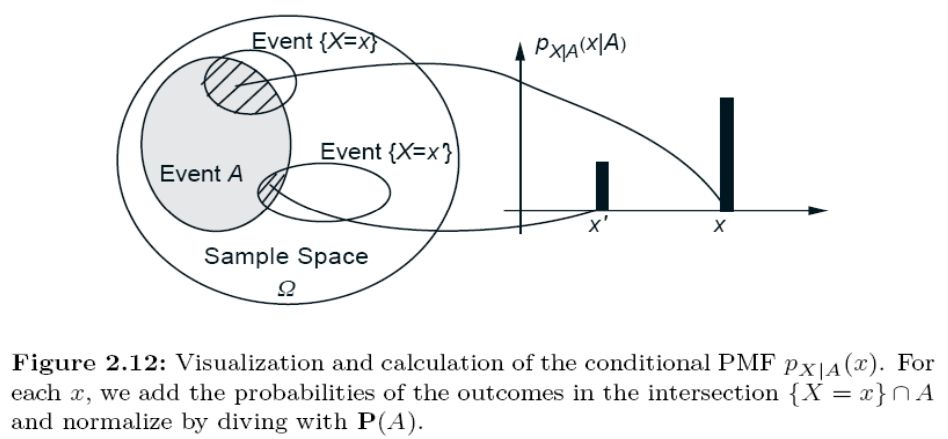
\includegraphics[width=.7\textwidth]{images/P_conditional_pmf.jpg}
 \end{figure}

 \subsection{Conditioning one \RV on another}
 If we are given that out of the two \rv $X$ and $Y$ that $Y=y$ has occurred with probability $p_Y(y)>0$ then it gives us partial knowledge about the value of $X$. This knowledge is captured by conditional PMF $p_{X|Y}$ of $X$ given $Y$, which is defined by the definition of $p_{X|A}$ to the events $A$ of the form $\{Y=y\}$
 \[p_{X|Y}(x|y)= P(X=x|Y=y)\]

 According to the definition of conditional probabilities
 \[p_{X|Y}(x|y)=\frac{P(X=x,Y=y)}{P(Y=y)} = \frac{p_{X,Y}(x,y)}{p_Y(y)}\]

 Fixing some $Y=y$, consider $p_{X|Y}(x|y)$ as a function of $x$. This function is a valid PMF for $X$ as it assigns a non-negative value for each outcome and these values add up to 1.

 The shape of $p_{X|Y}$ is similar to $p_{X,Y}$  except that it is divided by $p_Y(y)$ which enforces the normalization property ($\sum_x p_{X|Y}(x|y)=1$).

 We also have \[p_{X,Y}(x,y)=p_Y(y) p_{X|Y}(x|y) =p_X(x) p_{Y|X}(y|x)\]

 Conditional PMFs can be used to calculate marignal PMFs
 \[p_X(x)=\sum_y p_{X,Y}(x,y)=\sum_y p_Y(y)p_{X|Y}(x|y)\]

 This provides a divide and conquer method for calculating marignal PMFs and is similar in spirit to total probability theorum.

 If $A_1, \ldots, A_n$ are disjoint events that form a partition of the sample space ($P(A_i)>0$ for all $i$) then
 \[p_X(x)=\sum_{i=1}^{n} P(A_i) p_{X|A_i}(x)\]

 This is a special case of total probability theorum. Furthermore for any event $B$ with $P(A_i \cap B)>0$ for all $i$ then
 \[p_{X|B}(x)=\sum_{i=1}^n P(A_i|B)p_{X|A_i \cap B}(x)\]

 \subsection{Conditional Expectation}
 A conditional PMF can be thought of as an ordinary PMF over a new universe determined by the conditioning event. In the same spirit, a conditional expectation is the ordinary expectation except that it refers to the new universe, and all the probabilities and PMFs are replaced by their conditional counterparts.

 If $X$ and $Y$ are the two \rv associated with the same experiment
 \begin{enumerate}
     \item The conditional expectation of $X$ given an event $A$ with $P(A)>0$ is defined by
        \[\E[X|A]=\sum_x xp_{X|A}(x)\]
     for a function $g(X)$ we have
        \[\E[g(X)|A]=\sum_x g(x) p_{X|A}(x)\]
     \item The conditional expectation of $X$ that $Y$ takes a given $y$ is 
        \[\E[X|Y=y]=\sum_x x p_{X|Y}(x|y)\]
     \item If $A_1, \ldots, A_n$ be disjoint events that form a partition of the sample space ($P(A_i)>0$ for all $i$) then
        \[\E[X]=\sum_{i=1}^n P(A_i) \E[X|A_i]\]
    Furthermore for any event $B$ with $P(A_i \cap B)>0$ for all $i$ then
        \[\E[X|B]=\sum_{i=1}^n P(A_i|B)\E[X|A_i \cap B]\]
    \item We have \[\E[X]=\sum_y p_Y(y) \E[X|Y=y]\]
    \end{enumerate}

Last 3 equalities are equivalent and are therefore termed collectively as \textbf{total expectation theorum}. They all follow the idea that "The unconditional average can be obtained by averaging the conditional averages."

\subsubsection{Example: Geometric Mean and Variance}
Suppose that $X$ is a geometric \rv with PMF
\[p_X(k)=(1-p)^{k-1}p, \quad k=1,2,\ldots\]
The mean and variance is given by
\begin{align*}
    \E[X] &= \sum_{k=1}^{\infty} k (1-p)^{k-1} p \\
    \text{var}(X) &= \sum_{k=1}^{\infty}(k-\E[X])^2(1-p)^{k-1}p
\end{align*}
This is tedious to calculate. Let's think simpler.

If the first try is successful then we have $X=1$ and $\E[X|X=1]=1$. Otherwise we have wasted a trial and we are back at the same problem to be solved. Thus $\E[X|X>1]=1+\E[X]$.
Therefore 
\begin{align*}
    \E[X] &= P(X=1)\E[X|X=1] + P(X>1)(1+\E[X]) \\
         &= p + (1-p)(1+\E[X]) = \frac{1}{p} \\
\end{align*}

With a similar reasoning we have
\begin{align*}
    \E[X^2|X=1] &= 1 \\
    \E[X^2|X>1] &= \E[(1+X)^2] = 1 + 2\E[X]+\E[X^2] \\
    \E[X^2] &= p \cdot 1 + (1-p)(1+2\E[X]+\E[X^2]) \\
           &= \frac{1+2(1-p)\E[X]}{p} = \frac{2-p}{p^2} \\
    \text{var}(X)&= \E[X^2]-\E[X]^2=\frac{1-p}{p^2}
\end{align*}
\qed
\subsubsection{Example: Two Envelopes Paradox.}
See Example 2.18 (p. 106) \cite{intro-to-prob} if you're curious.

\section{Independence}
The concepts in this section will be analogous to the concepts of independence between events. They are developed by simply introducing suitable events involving the possible values of the random variable and by considering the independence of these events.

\subsection{Independence of a \RV from an Event}
Intuitively this means that the occurrence of an event provides does not provide any extra information on the likeliness of the different values that the \rv can take.

We say that a \rv is independent of an event $A$ if 
\[\boxed{P(X=x \text{ and } A)=P(X=x)P(A)=p_X(x)P(A)=p_{X|A}(x)P(A)} \qquad \forall x\]

This implies that for every value that the \rv can take the above equality must hold. As long as $P(A)>0$, independence is same as the condition
\[ \boxed{p_{X|A}(x) = p_X(x)} \qquad \forall x\]

\subsection{Independence of \RV}
We say that two \rv are independent if
\[\boxed{p_{X,Y}=p_X(x)p_Y(y)} \qquad \forall x,y\]

In case of conditioning event $A$ we have a new universe and the PMFs have to be replaced by the conditional counterparts. $X, Y$ are said to be conditionally independent given an positive probability event $A$, if

\[\boxed{P(X=x, Y=y | A) = p_{X|A}(x) p_{Y|A}(y)} \qquad \forall x,y\]

This is equivalent to 
\[p_{X|Y,A}(x|y)=p_{X|A}(x) \qquad \forall x,y \text{ such that } p_{Y|A}(y)>0\]

\begin{remark}
    In case of events conditional independence may not imply unconditional independence and vice versa.
\end{remark}

If two $X, Y$ are independent then 
\[\E[XY]=\E[X]\E[Y]\] 
\[ \boxed{\E[g(X)h(Y)]=\E[g(x)]\E[h(Y)]}\]

We have
\begin{center}
    var($X+Y$) = var($X$) $+$ var($Y$) \\
    var($X_1+\cdots+X_n$) = var($X_1$) $+ \cdots+$ var($X_n$) 
\end{center}

\subsection{Independence of several \RV}
Independence of several variables is a simple extension to the above discussion. If for $X, Y, Z$ the following condition holds
\[p_{X,Y,Z}=p_X(x)p_Y(y)p_Z(z)  \qquad \forall x,y,z\]
then the random variables are independent.
